\documentclass{article}
\usepackage{eason}

\usepackage{pdfpages}

\usepackage[a4paper, margin=1in]{geometry}

\usepackage{multicol}

\usepackage{lipsum}

\newcommand{\DATE}{dummyDate}
\newcommand{\COMMITSHA}{dummySHA}

\title{TMUA Lecture 2 -- Polynomials, Trigonometry and Geometry}
\author{Eason Shao}
\date{v.\DATE.\COMMITSHA}

\begin{document}
\maketitle

\tableofcontents

\section{Polynomials}
\subsection{Definition}
A \textbf{polynomial} is of the form
\[
    a_n x^n + a_{n - 1} x^{n - 1} + \cdots + a_1 x + a_0
\]
where \(n \geq 0\) is a natural number. Such \(n\) is called the \textbf{degree} of a polynomial. \(a_n, a_{n - 1}, \ldots, a_1, a_0\) are the \textbf{coefficients} of the polynomial. (We assume that they are real.)

\subsection{Polynomial Division and Factor Theorem}
\textbf{Polynomial division/remainder theorem} (Euclidean division) states that for any polynomial \(P\) (the polynomial to be divided) and \(D \neq 0\) (the \textbf{divisor}), there are two polynomials \(Q\) (the \textbf{quotient}) and \(R\) (the \textbf{remainder}), such that
\[
    P \pqty{x} = Q \pqty{x} D\pqty{x} + R \pqty{x}
\]
where \(\deg R < \deg D\).

\begin{problem}
    Can you try proving this? Which other number system allows for division with remainder like this? (There is a very deep reason behind this.)
\end{problem}

\begin{problem}
    If \(P\) and \(Q\) are polynomials in \(x\) with degree \(a\) and \(b\) respectively, what is the degree of \(P\pqty{x} + Q\pqty{x}\) and \(P\pqty{x}Q\pqty{x}\)? What about \(P\pqty{Q\pqty{x}}\)? (Do not forget degenerate cases!)
\end{problem}

\textbf{Long division} and \textbf{synthetic division} are computational methods to divide polynomials.

\begin{example}
    Divide the polynomial \(\pqty{x^4 + 2 x^3 + 3x + 5}\) by \(\pqty{x^2 + 2x + 1}\).
\end{example}

\textbf{Factor theorem} states that the remainder of a polynomial \(P\) upon division by \(\pqty{x - a}\) is a constant given by \(P\pqty{a}\).

\begin{proof}
    Write \(P\pqty{x} = \pqty{x - a} D\pqty{x} + R\pqty{x}\) and observe \(R\) has degree less than \(1\), hence constant. Plug in \(x = a\).
\end{proof}

\begin{example}[TMUA 2016 P1 Q2]
    The expression \(3 x^3 + 13 x^2 + 8x + a\), where \(a\) is a constant, has \(\pqty{x + 2}\) as a factor. Factorise this expression.
\end{example}

\begin{example}[TMUA 2017 P1 Q4]
    When \(\pqty{3 x^2 + 8x - 3}\) is multiplied by \(\pqty{px - 1}\) and the resulting product is divided by \(\pqty{x + 1}\), the remainder is \(24\). What is the value of \(p\)?
\end{example}

Some more challenging exercises sourced from the MAT:

\begin{example}[MAT 2013, Question G]
    Let \(n \geq 2\) be an integer and \(p_n \pqty{x}\) be the polynomial
    \[
        p_n \pqty{x} = \pqty{x - 1} + \pqty{x - 2} + \cdots + \pqty{x - n}.
    \]

    Find the remainder when \(p_n \pqty{x}\) is divided by \(p_{n - 1} \pqty{x}\).
\end{example}

\begin{example}[MAT 2009 Question I]
    For which values of \(n\) does the polynomial
    \[
        n^2 x^{2n + 3} - 25 n x^{n + 1} + 150 x^7
    \]
    have \(\pqty{x^2 - 1}\) as a factor?
\end{example}

\subsection{Roots of Polynomials}
\textbf{Fundamental Theorem of Algebra} states that for any degree-\(n\) complex polynomial \(P\pqty{x}\), it has \(n\) complex roots (including repeats), and hence can be factorised in the form
\[
    P\pqty{x} = a_n \pqty{x - x_1} \pqty{x - x_2} \cdots \pqty{x - x_n}.
\]

If \(P\) is a real polynomial, the roots \(x_1, \ldots, x_n\) may be complex, but complex roots come in conjugate pairs, so it can be factorised into linear and quadratic factors.

In practice, using this factorisation to determine how many real roots a polynomial has is very impracticable. Therefore, we analyse its stationary points and its increasing/decreasing property (i.e. analyse the sign of \(P'\pqty{x}\)) to determine the number of roots it has.

Recall the \textbf{intermediate value theorem} states that if \(\functiondomain{f}{\ccintv{a}{b}}{\RR}\) is continuous, with \(f\pqty{a} < 0\) and \(f\pqty{b} > 0\), then there is some \(c \in \oointv{a}{b}\) such that
\[
    f\pqty{c} = 0.
\]

Together with monotonicity, we may assert that such \(c\) is in fact unique.

\begin{problem}
    Problem for thinking: why does the intermediate value theorem hold?
\end{problem}

\begin{example}[TMUA 2016 P1 Q13]
    How many real roots does the equation \(3 x^5 - 10 x^3 - 120 x + 30 = 0\) have?
\end{example}

\begin{example}[TMUA 2016 P2 Q14]
    Let \(f\pqty{x} = a x^4 + b x^3 + c x^2 + d x + e\), where \(a, b, c, d\) and \(e\) are real numbers. Suppose \(f\pqty{x} = 1, 2, 3, 4\) has \(p, q, r, s\) solutions, respectively, which one of the following is \emph{not} possible?
    \begin{enumerate}
        \item \(\pqty{p, q, r, s} = \pqty{1, 2, 4, 3}\),
        \item \(\pqty{p, q, r, s} = \pqty{1, 3, 2, 4}\),
        \item \(\pqty{p, q, r, s} = \pqty{1, 4, 3, 2}\),
        \item \(\pqty{p, q, r, s} = \pqty{2, 4, 3, 1}\),
        \item \(\pqty{p, q, r, s} = \pqty{4, 3, 2, 1}\).
    \end{enumerate}
\end{example}

\begin{example}[TMUA 2017 P2 Q19]
    Which one of the following is a sufficient condition for the equation \(x^3 - 3 x^2 + a = 0\), where \(a\) is a constant, to have exactly one real root?
    \begin{enumerate}
        \item \(a > 0\)
        \item \(a \leq 0\)
        \item \(a \geq 4\)
        \item \(a < 4\)
        \item \(\abs{a} > 4\)
        \item \(\abs{a} \leq 4\)
        \item \(a = \frac{9}{4}\)
        \item \(\abs{a} = \frac{3}{2}\)
    \end{enumerate}
\end{example}

Some more exercises sourced from the MAT:
\begin{example}[MAT 2019, Question A]
    Find the number of real solutions to the equation \(x^3 - 300 x = 3000\).
\end{example}

\begin{example}[MAT 2009, Question F]
    For which values of \(k\) does the equation \(3 x^4 - 16 x^3 + 18 x^2 + k = 0\) have four real solutions in \(x\)?
\end{example}

\section{Trigonometric Functions}
\subsection{Radians}

The angle measured in \textbf{radians} is the ratio of the arc length to the radius of the circle.

By this definition, we have \(360 \degree = 2 \pi\), or equivalently \(180 \degree = \pi\). You probably want to memorise the radians of common angles, including:
\begin{multicols}{4}
    \begin{itemize}
        \item \(0 \degree = 0\)
        \item \(15 \degree = \flatfrac{\pi}{12}\)
        \item \(30 \degree = \flatfrac{\pi}{6}\)
        \item \(45 \degree = \flatfrac{\pi}{4}\)
        \item \(60 \degree = \flatfrac{\pi}{3}\)
        \item \(90 \degree = \flatfrac{\pi}{2}\)
        \item \(120 \degree = \flatfrac{2\pi}{3}\)
        \item \(135 \degree = \flatfrac{3\pi}{4}\)
        \item \(150 \degree = \flatfrac{5\pi}{6}\)
        \item \(180 \degree = \pi\)
        \item \(270 \degree = \flatfrac{3\pi}{2}\)
        \item \(360 \degree = 2 \pi\)
    \end{itemize}
\end{multicols}

\begin{problem}
    Is there another good reason why we should use radians? (Hint: differentiation)
\end{problem}

\subsection{Definitions}

Informally, for a point \(P\pqty{x, y}\) on the unit circle at angle \(\theta\) we may define the three trigonometric functions as:
\[
    \sin \theta = y, \quad \cos \theta = x
\]
and
\[
    \tan \theta = \frac{\sin \theta}{\cos \theta} = \frac{y}{x}.
\]

\(\sin\) and \(\tan\) has domain \(\RR\), image \(\ccintv{-1}{1}\), and period \(2 \pi\).

\(\tan\) has domain \(x \neq \frac{\pi}{2} + k \pi\), image \(\RR\), and period \(\pi\).

Special values from geometry:
\begin{multicols}{3}
    \begin{itemize}
        \item \(\sin 0 = \sin 0 \degree = 0\)
        \item \(\sin \pqty{\flatfrac{\pi}{6}} = \sin 30 \degree = \flatfrac{1}{2}\)
        \item \(\sin \pqty{\flatfrac{\pi}{4}} = \sin 45 \degree = \flatfrac{\sqrt{2}}{2}\)
        \item \(\sin \pqty{\flatfrac{\pi}{3}} = \sin 60 \degree = \flatfrac{\sqrt{3}}{2}\)
        \item \(\sin \pqty{\flatfrac{\pi}{2}} = \sin 90 \degree = 1\)
        \item \(\cos 0 = \cos 0 \degree = 1\)
        \item \(\cos \pqty{\flatfrac{\pi}{6}} = \cos 30 \degree = \flatfrac{\sqrt{3}}{2}\)
        \item \(\cos \pqty{\flatfrac{\pi}{4}} = \cos 45 \degree = \flatfrac{\sqrt{2}}{2}\)
        \item \(\cos \pqty{\flatfrac{\pi}{3}} = \cos 60 \degree = \flatfrac{1}{2}\)
        \item \(\cos \pqty{\flatfrac{\pi}{2}} = \cos 90 \degree = 0\)
        \item \(\tan 0 = \tan 0 \degree = 0\)
        \item \(\tan \pqty{\flatfrac{\pi}{6}} = \tan 30 \degree = \flatfrac{\sqrt{3}}{3}\)
        \item \(\tan \pqty{\flatfrac{\pi}{4}} = \tan 45 \degree = 1\)
        \item \(\tan \pqty{\flatfrac{\pi}{3}} = \tan 60 \degree = \sqrt{3}\)
        \item \(\tan \pqty{\flatfrac{\pi}{2}}, \tan 90 \degree\) \textbf{DNE}
    \end{itemize}
\end{multicols}

\begin{problem}
    What is the issue with this ``informal'' definition? How might a (pure) mathematician ``formally'' define it?
\end{problem}

\subsection{Graphs and Induction Formulae}

Trigonometric graphs not only have periodicity -- they also have symmetry properties built into them. (Below, all \(k\) are meant \(k \in \ZZ\).)

For the \(\sin\) function, it is symmetric about the lines \(x = \flatfrac{\pi}{2} + k \pi\), and rotationally symmetric (by \(180\degree\)) about the centres \(\pqty{k \pi, 0}\).

For the \(\cos\) function, it is symmetric about the lines \(x = k \pi\), and rotationally symmetric (by \(180\degree\)) about the centres \(\pqty{\flatfrac{\pi}{2} + k \pi, 0}\).

For the \(\tan\) function, it is not symmetric about any line, but it is rotationally symmetric (by \(180 \degree\)) about the centres \(\pqty{k \pi, 0}\).

Using these properties, we may reduce the sine/cosine of any angle to that within our familiar range of \(0\) to \(\flatfrac{\pi}{2}\). The best way to do so, and the way I always do this, is by looking at the graphs of the trigonometric functions.

\begin{examples}
    Find the \(\sin\) and \(\cos\) of the following angles, in terms of \(\sin \alpha\) or \(\cos \alpha\):
    \[
        \frac{\pi}{2} \pm \alpha, \quad \pi \pm \alpha, \quad \frac{3\pi}{2} \pm \alpha, \quad 2\pi \pm \alpha.
    \]
\end{examples}

\begin{examples}
    Find the following values:
    \begin{multicols}{4}
        \begin{itemize}
            \item \(\sin 120 \degree\)
            \item \(\cos 150 \degree\)
            \item \(\sin 390 \degree\)
            \item \(\cos 420 \degree\)
            \item \(\sin \pqty{\flatfrac{5\pi}{3}}\)
            \item \(\cos \pqty{\flatfrac{7\pi}{4}}\)
            \item \(\sin \pqty{\flatfrac{17\pi}{4}}\)
            \item \(\cos \pqty{- \flatfrac{13\pi}{6}}\)
        \end{itemize}
    \end{multicols}
\end{examples}

\subsection{Identities(y)}

The TMUA only requires this one, single formula for trigonometry, the Pythagorean Theorem:
\[
    \sin^2 x + \cos^2 x = 1.
\]

\begin{problem}
    How would you ``prove'' this identity? Is your proof tautological?
\end{problem}

Double angle formulae and addition formulae are not required in the syllabus, so if you see something involving \(\cos 2x\), you should probably not worry about expanding it.

\subsection{Solving Trigonometric Equations}

The eventual goal is to reduce the equation into the form
\[
    \sin \pqty{f\pqty{x}} = c,
\]
or \(\cos\), or \(\tan\), where \(f\) is a function of \(x\) that can be easily inverted.

For example, if you see a mix of \(\cos\) and \(\sin\) with squares, it is probably wise to use the Pythagorean Theorem to reduce to a problem with only \(\sin\) or only \(\cos\), ideally matching the linear term. In this case, it is often the case that the result will be a hidden quadratic (which solves to the result above).

Always draw a graph to solve for \(f\pqty{x}\) in the form above, noting especially that \textbf{the range we want to solve for \(f\pqty{x}\) might differ from the range of \(x\) itself}. Then apply \(f\inverse\) to your solution and \textbf{double-check your solution to \(x\) is within the desired range}. We want to make sure we don't ``over-solve'' or ``under-solve''!

\begin{examples}
    Solve the following trigonometric equations in the given range.
    \begin{itemize}
        \item \(\tan x = - \flatfrac{1}{\sqrt{3}}\) for \(-\pi < x < \pi\)
        \item \(\sin^2 \pqty{2x + \flatfrac{\pi}{3}} = \flatfrac{1}{2}\) for \(-2 \pi < x < 2\pi\)
        \item \(12 \cos^2 x + 6 \sin x - 10 = 2\) for \(0\degree < x < 360\degree\)
    \end{itemize}
\end{examples}

\begin{example}[TMUA 2016 P1 Q8]
    Find the maximum angle \(x\) in the range \(0\degree \leq x \leq 360\degree\) which satisfies the equation
    \[
        \cos^2 \pqty{2x} + \sqrt{3} \sin \pqty{2x} - \frac{7}{4} = 0.
    \]
\end{example}

\begin{example}[TMUA 2016 P1 Q17]
    It is given that
    \[
        y = \pqty{1 + 2 \cos x} \cos 2x \qfor 0 < x < \pi
    \]

    Find the complete set of values of \(x\) for which \(y\) is negative.
\end{example}

\begin{example}[TMUA 2016 P2 Q3]
    What is the value, in radians, of the largest angle \(x\) in the range \(0 \leq x \leq 2\pi\) that satisfies the equation \(8 \sin^2 x + 4 \cos^2 x = 7\)?
\end{example}

\begin{example}[TMUA 2017 P1 Q8]
    Find the complete set of values of \(x\), with \(0 \leq x \leq \pi\), for which
    \[
        \pqty{1 - 2 \sin x} \cos x \geq 0.
    \]
\end{example}

\begin{example}[TMUA 2017 P2 Q4]
    The following question appeared in an examination:

    \indent Given that \(\tan x = \sqrt{3}\), find the possible values of \(\sin 2x\).

    A student gave the following answer:

    \indent \(\tan x = \sqrt{3}\) so \(x = 60 \degree\) and \(2x = 120 \degree\), therefore \(\sin 2x = \dfrac{\sqrt{3}}{2}\)

    Which one of the following statements is correct?

    \begin{enumerate}
        \item \(\dfrac{\sqrt{3}}{2}\) is the only possible value, and this is fully supported by the reasoning given in the student's answer.
        \item \(\dfrac{\sqrt{3}}{2}\) is the only possible value, but the reasoning given should consider other possible values of \(x\) for which \(\tan x = \sqrt{3}\).
        \item \(\dfrac{\sqrt{3}}{2}\) is the only possible value, but the reasoning given should consider other possible values of \(x\) for which \(\sin 2x = \dfrac{\sqrt{3}}{2}\).
        \item \(\dfrac{\sqrt{3}}{2}\) is \textbf{not} the only possible value because the reasoning given should have considered other possible values of \(x\) for which \(\tan x = \sqrt{3}\).
        \item \(\dfrac{\sqrt{3}}{2}\) is \textbf{not} the only possible value because the reasoning given should have considered other possible values of \(x\) for which \(\sin 2x = \dfrac{\sqrt{3}}{2}\)
    \end{enumerate}
\end{example}

\begin{example}[TMUA 2017 P2 Q12]
    \autoref{fig:tmua-2017-p2-q12} shows the graphs of \(y = \sin 2x\) and \(y = \cos 2x\) for \(- \frac{\pi}{2} < x < \frac{\pi}{2}\).

    Which one of the following is \textbf{not} true?
    
    \begin{enumerate}
        \item \(\cos 2x < \sin 2x < \tan x\) for some real number \(x\) with \(- \frac{\pi}{2} < x < \frac{\pi}{2}\)
        \item \(\cos 2x < \tan x < \sin 2x\) for some real number \(x\) with \(- \frac{\pi}{2} < x < \frac{\pi}{2}\)
        \item \(\sin 2x < \cos 2x < \tan x\) for some real number \(x\) with \(- \frac{\pi}{2} < x < \frac{\pi}{2}\)
        \item \(\sin 2x < \tan x < \cos 2x\) for some real number \(x\) with \(- \frac{\pi}{2} < x < \frac{\pi}{2}\)
        \item \(\tan x < \sin 2x < \cos 2x\) for some real number \(x\) with \(- \frac{\pi}{2} < x < \frac{\pi}{2}\)
        \item \(\tan x < \cos 2x < \sin 2x\) for some real number \(x\) with \(- \frac{\pi}{2} < x < \frac{\pi}{2}\)
    \end{enumerate}
\end{example}

\begin{figure}[h!]
    \centering
    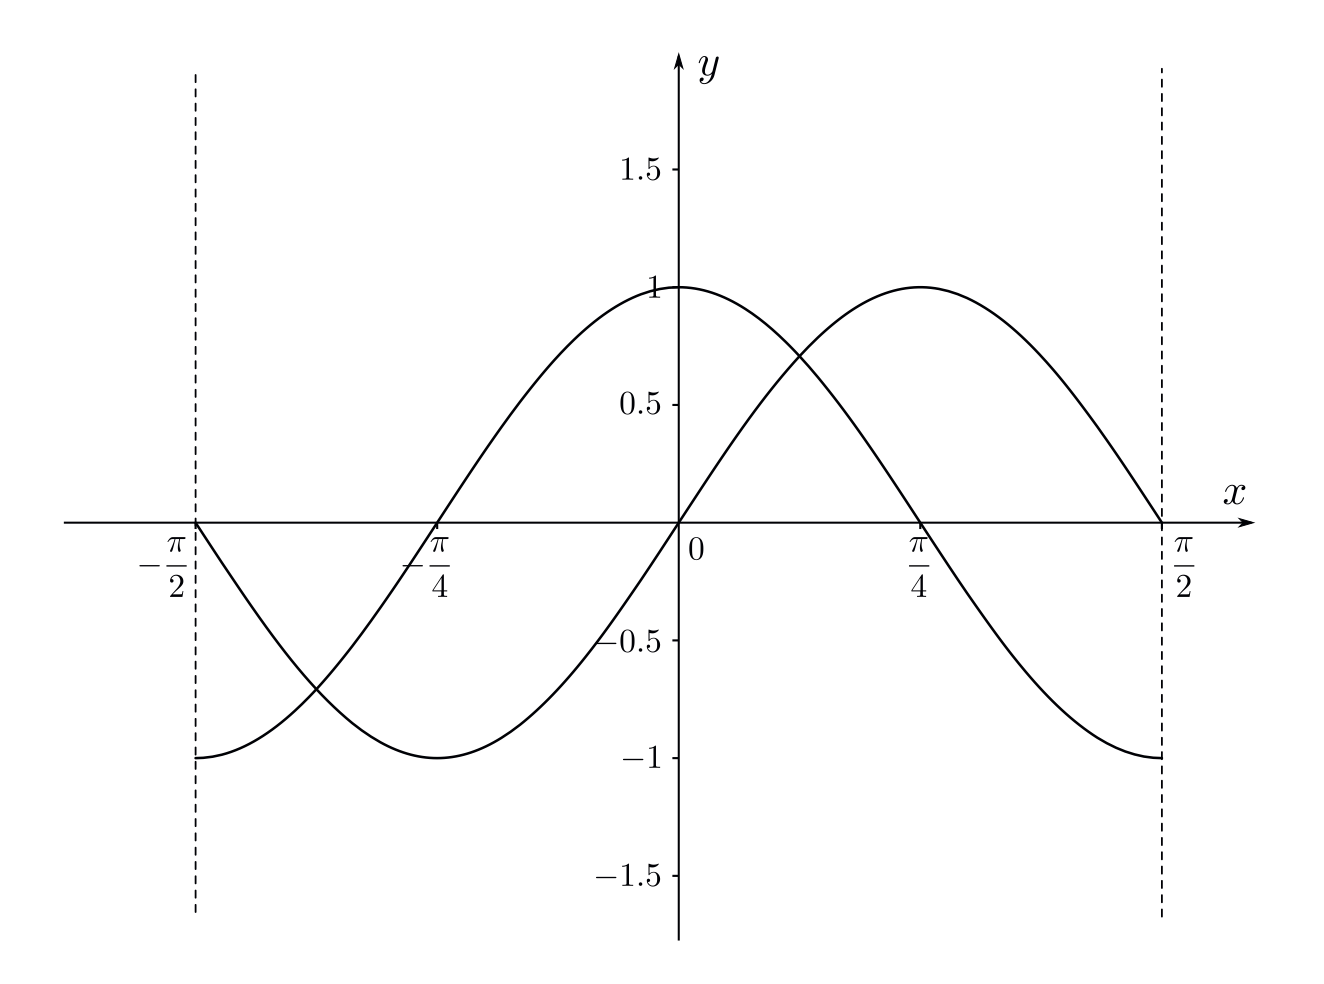
\includegraphics[width=0.8\linewidth]{tmua-2017-p2-q12.png}
    \caption{TMUA 2017 P2 Q12}
    \label{fig:tmua-2017-p2-q12}
\end{figure}

\section{Geometry in Triangles}
\subsection{Area Formulae, Sine Rule and Cosine Rule}
The very basic one: \(A = \frac{1}{2} ah\).

Area formula in the form of sine:
\[
    A = \frac{1}{2} ab \sin C = \frac{1}{2} ac \sin B = \frac{1}{2} bc \sin A.
\]

Another (potentially) useful one: Heron's formula which states
\[
    A = \sqrt{s \pqty{s - a} \pqty{s - b} \pqty{s - c}}
\]
where \(s = \frac{a + b + c}{2}\).

\begin{problem}
    Prove Heron's formula.
\end{problem}

Sine rule:
\[
    \frac{a}{\sin A} = \frac{b}{\sin B} = \frac{c}{\sin C}.
\]

\textbf{Note that the sine rule always solves for two possible values of an angle, due to the shape of the sine curve.} Sometimes, only one of those angles make sense, while for some other cases, there might be multiple possible triangles (``ambiguity'', see below).

\textbf{When to use sine rule:}
\begin{itemize}
    \item given two angles and one side, find the remaining angle and any other side;
    \item given two sides and one angle but not between them, find another angle.
\end{itemize}

Note: the second case gives rise to ``ambiguity'', see below.

Cosine rule:
\begin{align*}
    a^2 &= b^2 + c^2 - 2bc \cos A \\
    b^2 &= c^2 + a^2 - 2ca \cos B \\
    c^2 &= a^2 + b^2 - 2ab \cos C
\end{align*}

A useful rearrangement of the cosine rule:
\begin{align*}
    \cos A &= \frac{b^2 + c^2 - a^2}{2bc} \\
    \cos B &= \frac{c^2 + a^2 - b^2}{2ca} \\
    \cos C &= \frac{a^2 + b^2 - c^2}{2ab}
\end{align*}

\textbf{When to use cosine rule:}
\begin{itemize}
    \item given three sides, find any angle; (rearrangement)
    \item given two sides and the angle between them, find the third side. (original form)
\end{itemize}

\begin{problem}
    Prove the sine rule and cosine rule.
\end{problem}

\begin{example}[TMUA 2016 P1 Q20]
    The diagram in \autoref{fig:tmua-2016-p1-q20} shows a square-based pyramid with base \(PQRS\) and vertex \(O\). All the edges of the pyramid are of length \(20\) metres.

    Find the shortest distance, in metres, along the outer surface of the pyramid from \(P\) to the midpoint of \(OR\).
\end{example}

\begin{figure}[h!]
    \centering
    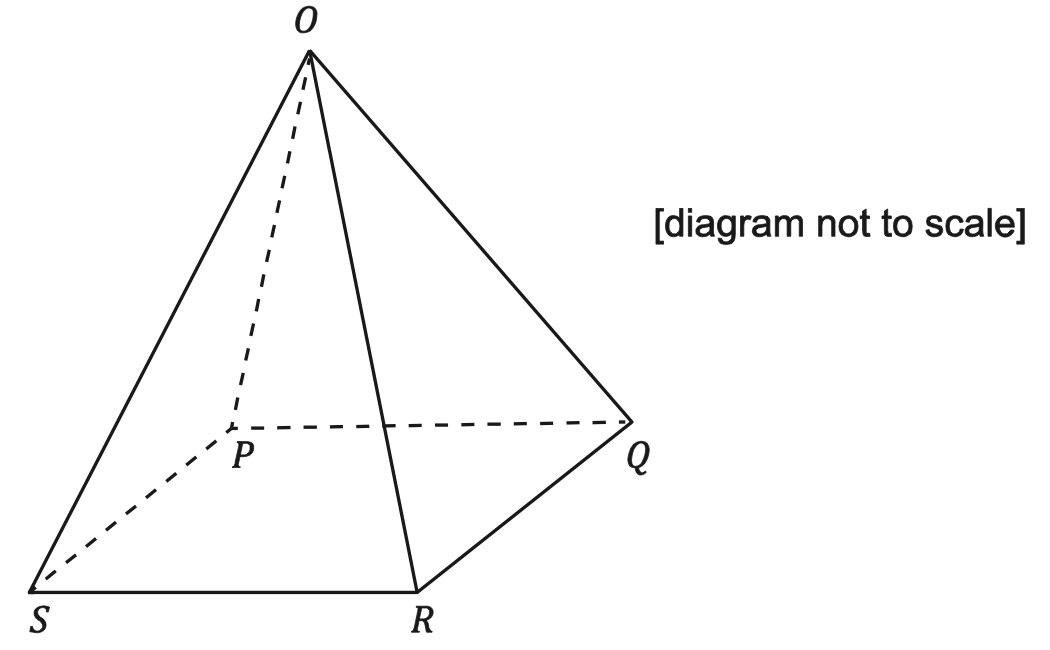
\includegraphics[width=0.7\linewidth]{tmua-2016-p1-q20.png}
    \caption{TMUA 2016 P1 Q20}
    \label{fig:tmua-2016-p1-q20}%
\end{figure}

\subsection{Congruence and Similarity}

\textbf{Congruence} is when two shapes are of the exact same dimensions (i.e. of the exact same shape and size). \textbf{Similarity} is when two shapes are of the same shape (but not necessarily the same size).

Formally speaking, \textbf{congruence} of polygons are when all the edges and the angles correspond (to be equal), while \textbf{similarity} of polygons are when the edges correspond to form a common ratio, and the angles correspond to be equal.

Therefore, congruence is \textbf{strictly a subset} of similarity.

Below, we restrict our view to triangles.

\textbf{Proving congruence from similarity} is by finding any useful information of the size of the triangle, e.g. the length of an edge, or the area of the triangle.

\textbf{Proving similarity} is by:
\begin{itemize}
    \item finding two angles which correspond to be equal (and the third must therefore be);
    \item having all three pairs of edges to be in common ratio;
    \item having two pairs of edges to be in common ration, and the angle in between them to be equal.
\end{itemize}

\textbf{Proving congruence} is by:
\begin{itemize}
    \item \textbf{SSS.} All three sides are equal.
    \item \textbf{SAS.} Two sides and an angle between them.
    \item \textbf{AAS/ASA.} A side and any two angles.
    \item \textbf{RHS.} Right-angled triangle, hypotenuse and any other side (which allows us to find the final side by Pythagorean Theorem).
\end{itemize}

\textbf{SSA} does not necessarily imply congruence -- see ``ambiguity'' case below.

\begin{example}[TMUA 2016 P2 Q9]
    Triangles \(ABC\) and \(XYZ\) have the \textbf{same area}.

    Which of these extra conditions, taken independently, would \textbf{imply} that they are congruent?

    \begin{enumerate}
        \item \(AB = XY\) \textbf{and} \(BC = YZ\)
        \item \(AB = XY\) \textbf{and} \(\angle ABC = \angle XYZ\)
        \item \(\angle ABC = \angle XYZ\) \textbf{and} \(\angle BCA = \angle YZX\)
    \end{enumerate}
\end{example}

\begin{example}[TMUA 2016 P2 Q16]
    In \autoref{fig:tmua-2016-p2-q16}, \(PQRS\) is a trapezium with \(PQ\) parallel to \(SR\). The diagonals of the trapezium meet at \(X\). \(U\) lies on \(SP\) and \(T\) lies on \(RQ\) such that \(UT\) is a line segment through \(X\) parallel to \(PQ\).

    The length of \(PQ\) is \(\SI{12}{\centi\metre}\) and the length of \(SR\) is \(\SI{3}{\centi\metre}\). What, in centimetres, is the length of \(UT\)?
\end{example}

\begin{figure}[h!]
    \centering
    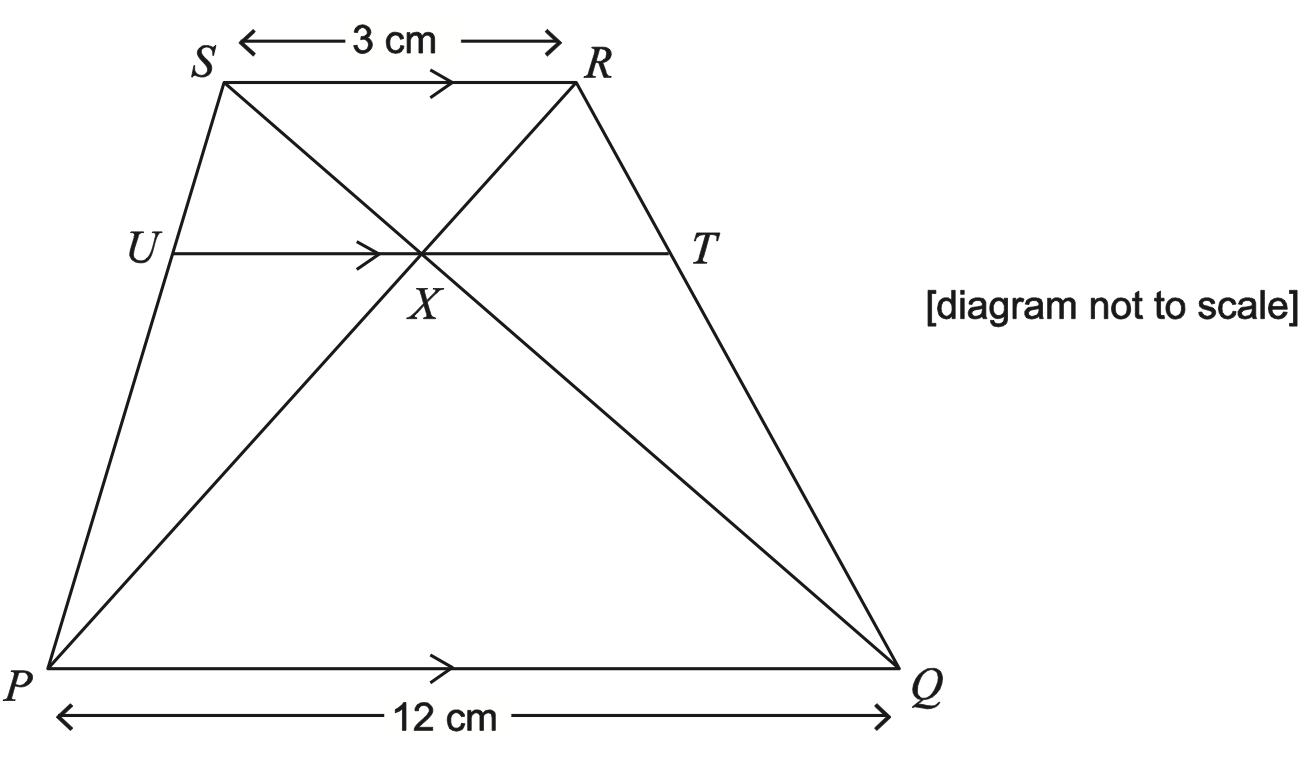
\includegraphics[width=0.8\linewidth]{tmua-2016-p2-q16.png}
    \caption{TMUA 2016 P2 Q16}
    \label{fig:tmua-2016-p2-q16}
\end{figure}

\begin{example}[TMUA 2017 P1 Q20]
    The lengths of the sides \(QR\), \(RP\) and \(PQ\) in triangle \(PQR\) are \(a\), \(a + d\) and \(a + 2d\) respectively. where \(a\) and \(d\) are positive and such that \(3d > 2a\).

    What is the full range, in degrees, of possible values for the angle \(PRQ\)?
\end{example}

\subsection{``Ambiguity'' Case}

\end{document}